\subsection{Sharding, conceptos generales}

Sharding es el proceso de almacenar datos a lo largo de múltiples máquinas y es la herramienta a través de la 
cual MongoDB combate el crecimiento de la demanda de datos. A medida que el tama\~no de los mismos aumenta,
una única máquina puede no ser suficiente para almacenar y proveer rates de lectura y escritura aceptables.
Sharding resuelve el problema de escalamiento horizontal. Se agregan más máquinas para soportar el crecimiento
de los datos y la demanda de usuarios de la base de datos.

Por el contrario, escalamiento vertical agrega más CPU y memoria para incrementar la capacidad. Escalar a través
del aumento de los recursos de una única máquina tiene sus limitaciones: Los sistemas de alta performance con
gran cantidad de CPU's y memoria RAM son desproporcionadamente más costosos que un conjunto de sistemas 
peque\~nos. En suma, los proveedores basados en la nube únicamente proveen instancias peque\~nas a los
usuarios. Como resultado, hay un tope máximo en la capacidad de escalar a nivel vertical.

Por el contrario, sharding o escalamiento horizontal, divide el set de datos y lo distribuye a lo largo de 
múltiples servidores. Cada shard es una base de datos independiente, y colectivamente, los shards conforman
una única lógica base de datos.

MongoDB sharding-guide.

\subsection{Sharding en MongoDB}

MongoDB soporta sharding a través de estructuras llamadas \emph{sharded clusters},
que cuentan con los siguientes componentes:

\begin{itemize}
	\item Shards o \emph{mongods}
	\item Query routers o \emph{mongos}
	\item Config servers 
\end{itemize}

Shards o \emph{mongods} son los nodos de almacenamiento de datos. Cada nodo está compuesto por un 
conjunto replicado (\emph{replica set}). 
Los Query routers o \emph{mongos} actúan de intermediarios entre los pedidos de los clientes y los shards correspondientes
que contienen esos datos específicos. Un cluster puede contener más de un query router (y es conveniente que así) sea,
para disminuír cantidad de pedidos que debe manejar un único nodo.
Finalmente, los Config servers almacenan la metadata del cluster: principalmente, el mapeo de los datos en cada uno de los
shards.

\subsection{Decisiones de arquitectura}

Para establecer la base de datos de \emph{Rededit} tomamos las siguientes decisiones de arquitectura:

\subsubsection{\emph{Shards y Replica sets}}

Cada \emph{shard} está constituida por un \emph{replica set}: un conjunto de nodos que mejoran la 
disponibilidad de los datos del
servidor en base a la redundancia. Existen tres tipos de miembros:

\begin{description}
	\item[Primario] Recibe las operaciones de escritura.
	\item[Secundario] Replican las mismas operaciones efectuadas por el primario para mantener el set de datos consistente.
	\item[Árbitro] Opcional. 
	No almacena datos. Simplemente participa en la elección de un nuevo nodo primario en los casos en donde el actual se
	encuentra inhabilitado.
\end{description}

Decidimos adoptar una de las configuraciones típicas propuestas en \emph{MongoDB-replication-guide}: 
Una estructura conformada por tres nodos, todas ellas almacenando datos: 

~

\begin{description}
	\item[Uno primario] 
	\item[Dos secundarios] Ambos son candidatos a volverse primarios luego de una elección, en el caso de una falla
	en el nodo primario.
	\item[Ningún árbitro]
\end{description}

~

Mediante esta elección disponemos de 2 copias completas del set de datos además del primario. Provee tolerancia a fallos
en el nodo primario, y buena velocidad de respuesta debido a la redundancia.

\subsubsection{Config servers}

El cluster va a contar con 3 servidores de configuración (Cantidad sugerida por \emph{MongoDB-sharding-guide}).

\subsection{\emph{Mongos y shards}}

El cluster cuenta inicialmente con 2 \emph{mongos} o query routers y 2 shards (cluster minimal de MongoDB). La idea es
ir incrementando la cantidad de nodos a medida que aumente la cantidad de usuarios de
la aplicación, y por lo tanto, las necesidades de nuestro servidor para satisfacer exitosamente todos los pedidos.

\begin{figure}[!h]
	\begin{center}
		  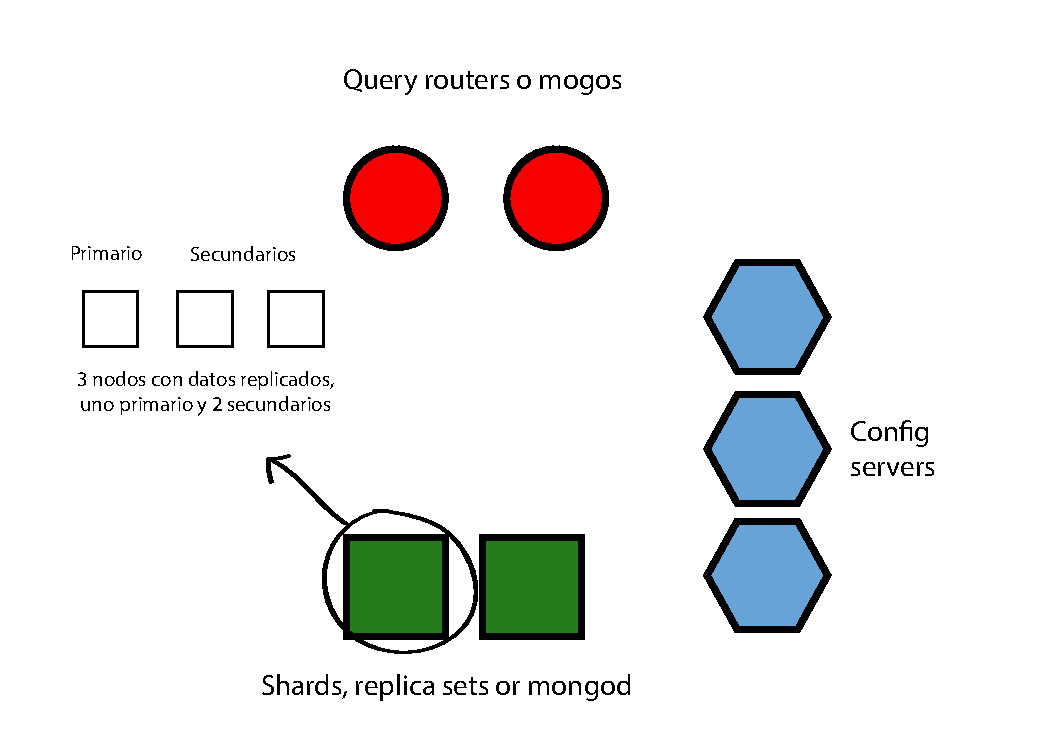
\includegraphics[scale=0.6]{imagenes/im_3.pdf}
		  \caption{Arquitectura inicial con la que empieza la base de datos de mongoDB}
		  \label{fig:contra1}
	\end{center}
\end{figure}
\FloatBarrier

\subsection{Incremento de Mongos y shards}

Finalmente hemos tomado la siguiente decisión para determinar el momento de aumentar o disminuír la cantidad de nodos
de nuestro cluster.

Cuando los datos almacenados alcanzan $\frac{3}{4}$ de 
la capacidad total de almacenamiento de nuestro servidor (suma de las capacidades de los shards) 
duplicamos la cantidad de shards del cluster.

Si por el contrario, los datos almacenados disminuyen a menos de $\frac{1}{4}$ de la capacidad total (por ejemplo,
debido a la baja del sistema de muchos de los usuarios), entonces reducimos a la mitad la cantidad de shards.

Algo similar sucederá con la cantidad de \emph{mongos} o query routers del cluster. En cuanto el sistema detecte que
el tiempo de respuesta ante los pedidos de los usuarios es lento duplicamos la cantidad de routers, ya que la 
cntidad actual no logran satisfacer las demandas de los clientes. En el caso de que haya gran cantidad de query routers
que no procesan ningún pedido (los pedidos se distribuyen de manera uniforme entre los \emph{mongos}, cuando
la base está bien balanceada), es momento de reducir a la mitad la cantidad de query routers.

